\chapter{Convolution and the DFT}
The DFT diagonalizes convolutions.
Throughout, let \(S \in\mathbb{C}^N\) be the left circular shift matrix defined by
% \begin{align}
  \((Sx)[n] = x[n+1]\),
  % \intertext{
  where circular indexing is understood.
% \end{align}

% \section{Eigendecomposition of circular shift}
\begin{lemma}[Eigendecomposition of circular shift]
  The eigenvectors of \(S\) are the DFT basis vectors, and that the eigenvalues are the roots of unity.\footnote{We could just verify this directly, but I find that diagonalizing \(S\) helps to clarify the magic surrounding the DFT basis.}
\end{lemma}
\begin{proof}
To show this, suppose we have an eigenvalue-eigenvector pair
\begin{align}
  Sv &= \lambda v.
  \intertext{Multiplying through by \(S^{N-1}\),}
  S^N v &= \lambda S^{N - 1} v = \lambda^2 S^{N-2} v = \ldots = \lambda^N v.
  \intertext{On the left, \(S^N = I\) as \(N\) rotations amount to a revolution.}
  v &= \lambda^N v \\
  \del{\lambda^N - 1} v &= 0
  \intertext{As \(v\) is nonzero by virtue of being an eigenvector, by the zero product property,}
  \lambda^N &= 1\\
  \lambda &= \omega_N^0, \omega_N^1, \ldots, \omega_N^{N - 1}
  \intertext{Let's solve for \(u_k\), the eigenvector corresponding to \(\omega^k\).}
  S u_k &= \omega^k u_k \\
  % \intertext{At position \(n + }
  u_k[n + 1] &= \omega^k u_k[n]
  % \intertext{This so}
\end{align}
This shows that \(u_k\) consists of consecutive powers of \(\omega^k\).
Normalizing by \(\del{\sqrt{N}}^{-1}\) we have the DFT basis.
\end{proof}

% The eigenvalues of \(S\) are the \(N\)th roots of unity are the essence of all things \(N\)-periodic.

% \section{Interlude: matrix polynomials}
A \textbf{polynomial} in the indeterminate \(z\) is an expression of the form
\(p(z) = \sum_{k = 0}^{d} p_k z^k\), where \(d \geq 0\).
When \(p(z)\) is evaluated at a matrix \(A\), we use \(A^0 = I\).
\begin{lemma}[Eigendecomposition of a matrix polynomial]
  % \tag{lemma:matpol}
  Let \(A \in\mathbb{C}^{n\times n}\), and let \(p(z)\) be a polynomial in the indeterminate \(z\).
  Then if \(Av = \lambda v\) is an eigenvalue-eigenvector pair,
  then \(p(A) v = p(\lambda) v\).
\end{lemma}
\begin{proof}
  Let \(d\) be the degree of \(p\).
  \begin{align}
    p(A) v &= \sum_{k=0}^{d} p_k A^k v\\
    \intertext{It can be shown by induction on \(k\) that \(A^k v = \lambda^k\)v.}
    p(A) v &= \sum_{k=0}^{d} p_k \lambda^k v \\
    &= \del{\sum_{k=0}^{d} p_k \lambda^k} v\\
    &= p(\lambda) v
  \end{align}
  Therefore \(p(A)\) has the same eigenvectors as \(A\), but the eigenvalues are \(p(\lambda)\) for each eigenvalue \(\lambda\) of \(A\).
\end{proof}

\subsection{Example: Cayley-Hamilton theorem}
We can use calculus to show that if \(\chi\) is the characteristic polynomial of \(A\in\mathbb{C}^{n\times n}\), then \(\chi(A) = 0\).
First, if \(A\) is diagonalizable, then for every eigenvalue-eigenvector pair
\(A v = \lambda v\), we have \(\chi(A) v = \chi(\lambda) v = 0v\).
The matrix \(\chi(A)\) annihilates the eigenvectors of \(A\), which are a basis for \(\mathbb{C}^N\). Therefore \(\chi(A) = 0\).

If \(A\) is not diagonalizable, then let \(A = U M U^*\), where \(M\) is upper triangular and \(U\) is unitary.
Let \(D\) be a diagonal matrix such that \((M+\epsilon D)\) has no repeated diagonal elements for all sufficiently small \(\epsilon > 0\).
Let \(A_\epsilon = U\del{M + \epsilon}U^*\).
Then \(\chi_A(A) = \lim_{\epsilon \to 0} \chi_{A_\epsilon}(A_\epsilon)\).
For all \(\epsilon > 0\), \(A_\epsilon\) is diagonalizable and therefore vanishes under its own characteristic polynomial.
As polynomial functions are continuous, therefore \(\chi_A(A) =0 \).
% For every \(\epi

\subsection{Example: heat equation on a ring}
Let \(x[t] \in \mathbb{R}^N\) represent the temperatures of a solid ring, sampled at evenly spaced intervals.
According to the heat equation\footnote{Solved by Fourier using a continuous-time analog of the DFT.}, \(x\) evolves according to the following law:
\begin{align}
  x[t+1] &= A x[t], \quad \text{where} \\
  A &= \frac{1}{4}(2I + S + S^{N-1}).
  \intertext{\(A\) may be written as \(p(S)\), where \(p\) is the following polynomial:}
  p(z) &= \frac{1}{4}(2 + z + z^{N-1})
  \intertext{Therefore the eigenvectors of \(A\) are the DFT basis vectors, and the eigenvalues of \(A\) are}
  p(\omega_N^k)
  &= \frac{1}{4}(2 + \omega_N^k + \omega_N^{-k}) = \frac{1}{2}\del{1 + \cos{2\pi k/N}},
\end{align}
and this system is marginally stable.


\section{\(H\) is polynomial in \(S\), and a lot of conclusions}
If \(y = Hx\) for \(x,y \in\mathbb{C}^N\) is a linear time-invariant system with impulse response \(h\),
 then \(H\) is constant along stripes parallel to the diagonal.
 Decomposing \(H\) into its \(N\) stripes,
\begin{align}
  H &= \sum_{k=0}^{N-1} h[k] S^{-k}
  \intertext{Multiplying by \(S^N = I\),}
   &= \sum_{k=0}^{N-1} h[k] S^{N -k}\\
  &= \sum_{k=0}^{N-1} h[k] S^{N -k}\\
  &= p(S),\ \text{where}\
  \ p(z) = \sum_{k=0}^{N-1} h[k] z^{N- k}.\\
  \intertext{Therefore \(H\), being a polynomial in \(S\), has the same eigenvectors as \(S\). The DFT basis vector \(u_k\) satisfies \(Su_k = \omega_N^k u_k\), so it is also an eigenvector of \(H\) with eigenvalue \(p(\omega_N^k)\):}
  H u_k &= p(\omega^k) u_k
  \intertext{Let's find out what our eigenvalue \(p(\omega^k)\) is.}
  p(\omega^k)
  &= \sum_{\ell=0}^{N-1} h[\ell] \omega^{k(N- \ell)}
  \intertext{It's row \(k\) of the DFT analysis equation! Using the DFT}
  g &= Fh,\\
  \intertext{we have}
  p(\omega^k) &= \sqrt{N} g[k].
  \intertext{Therefore \(H\) has the following eigendecomposition:}
  H
  &= F^*
   G
  F =
  F^* \operatorname{diag}\{g\} F\\
  &=
  F^*
  \begin{pmatrix}
    \sqrt{N} g[0]      &   &    \\
     & \sqrt{N}  g[1] \\
     &                 & \ddots &\\
     &                &         & \sqrt{N} g[N-1]
  \end{pmatrix}
  F.
  \intertext{In the DFT basis, time domain convolution is represented as a pointwise multiplication (using the symbol \(\odot\)).}
  Fy &= \del{\sqrt{N} Fh} \odot Fx
\end{align}
Efficient algorithms for DFT and inverse DFTs can take advantage of the fact that \(F\) and \(F^*\) are symmetric matrices.
They run as fast as an efficient sorting algorithm.

\section{Square wave transmission, revisited}
\subsection{An indeterminate matrix limit}
We derived that the convolution matrix of a transmission line with time constant \(\tau\) is
\begin{align}
  H &= \del{1 - e^{-T/\tau}} \del{S - e^{-T/\tau} I} ^{-1}.
  \intertext{We showed that as \(\tau\to0\), \(H\to S^{-1}\), a one-sample delay.
  As \(\tau\to \infty\), \(\del{1 - e^{-T/\tau}} \to 0\), we have a ``0/0'' limit.}
  H_\text{slow}
  &= \lim_{\epsilon \to 0} \epsilon \del{S - \del{1-\epsilon} I}^{-1}
  \intertext{Diagonalize \(S\) as \(S = F^* \Omega F\), where \(\Omega = \operatorname{diag}\left\{\omega_N^0, \omega_N^1, \ldots, \omega_N^{N-1}\right\}\).}
  &= \lim_{\epsilon \to 0} \epsilon \del{F^*\Omega F - \del{1-\epsilon} I}^{-1}\\
  &= \lim_{\epsilon \to 0}
  \epsilon \del{F^*\del{\Omega  - \del{1-\epsilon} I}F}^{-1} \\
  &= \lim_{\epsilon \to 0}
  F^*\del{\frac{\Omega  - \del{1-\epsilon} I}{\epsilon}}^{-1}F \\
  &= \lim_{\epsilon \to 0}
  F^*
  \operatorname{diag}\left\{
    \frac{\epsilon}{\omega_N^0 - 1 + \epsilon},
    \frac{\epsilon}{\omega_N^1 - 1 + \epsilon}, \ldots,
    \frac{\epsilon}{\omega_N^{N-1} - 1 + \epsilon}
  \right\}
  F \\
  &= \lim_{\epsilon \to 0}
  F^*
  \operatorname{diag}\left\{
    \frac{\epsilon}{\epsilon},
    \frac{\epsilon}{\del{\text{nonzero}}}, \ldots,
    \frac{\epsilon}{\del{\text{nonzero}}}
  \right\}
  F \\
  &=
  F^*
  \operatorname{diag}\left\{1, 0, \ldots, 0 \right\}
  F \\
  &=
  \frac{1}{N}
  \begin{pmatrix}
    1 & \cdots & 1 \\
    \vdots & \ddots & \vdots \\
    1 & \cdots & 1 \\
  \end{pmatrix}
\end{align}
As our transmission line becomes infinitely slow, eventually it becomes impossible to move the output at all, and all AC signals are shorted through the parasitic shunt capacitor.
Only the DC component of the input passes.

\subsection{Input, transfer function, output}

\begin{figure}
  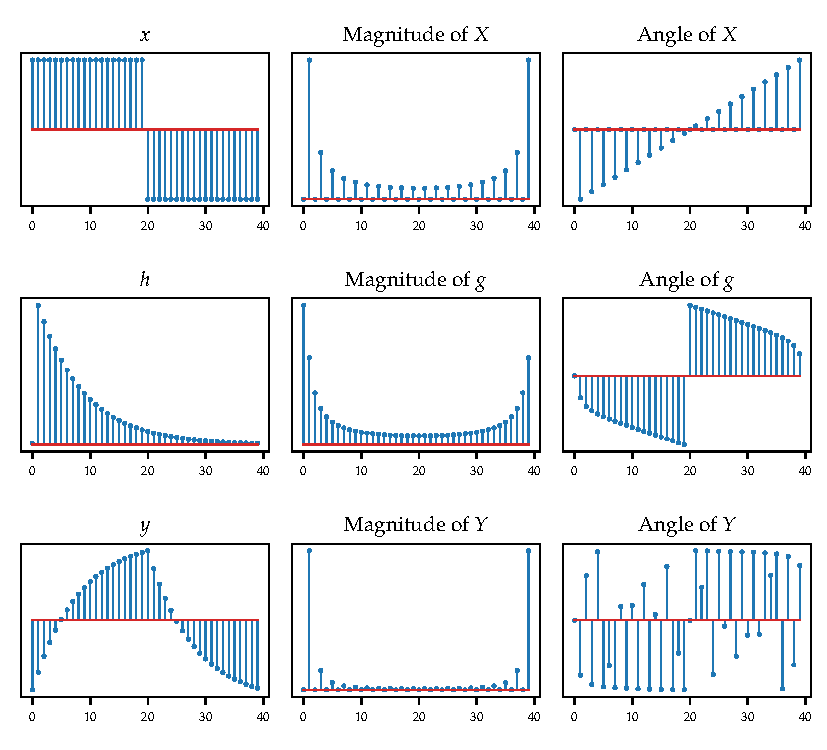
\includegraphics{27-figs/inHout}
  \caption{Input, impulse response, and output in time and frequency domain.}
  \label{fig:lec27-inHout}
\end{figure}
The left column of Figure~\ref{fig:lec27-inHout} shows:
\begin{itemize}
  \item \(x\), the square wave on the near end of the transmission line;
  \item \(h\), the impulse response of the transmission line; and
  \item \(y\), the output on the far end of the transmission line.
\end{itemize}
We showed that \(y\) is the convolution of \(x\) with \(h\).

The center and right columns of Figure~\ref{fig:lec27-inHout} show:
\begin{itemize}
  \item \(X= Fx\), the ``phasor'' representation of \(x\) in the DFT basis (note that \(x\) has only odd frequencies);
  \item \(g = Fx\), the ``transfer function'' representation of \(h\) in the DFT basis (can you tell that \(g\) is a low-pass filter?); and
  \item \(Y = \sqrt{N} g \odot X\), the ``phasor'' representation of \(y\) in the DFT basis. (When eyeballing \(g \odot X\), remember that magnitudes multiply and phases add.)\footnote{The phase of \(Y\) is crazy; don't think too hard about what it means.}
\end{itemize}

\subsection{Equalization using DFT}
\begin{figure}
  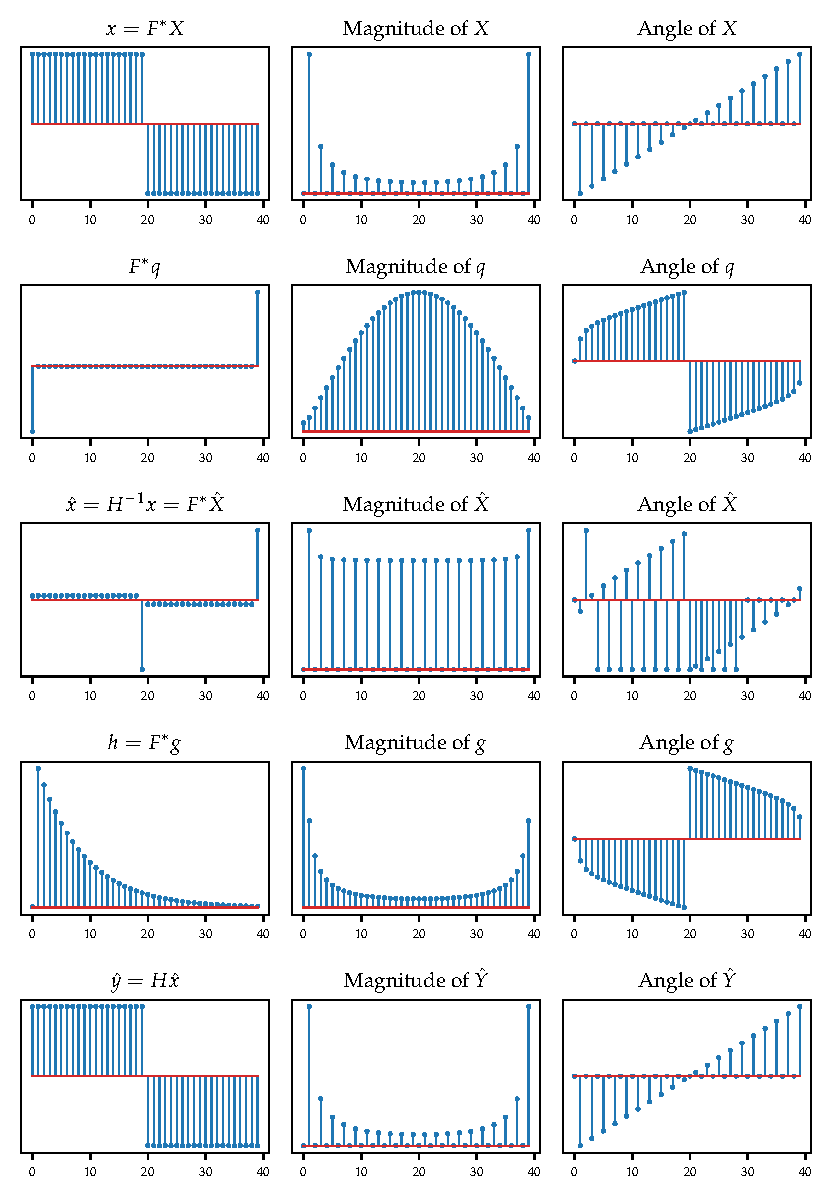
\includegraphics{27-figs/eq}
  \caption{Input, impulse response, and output in time and frequency domain.}
  \label{fig:lec27-eq}
\end{figure}

The transmission equation
\begin{align}
  y &= Hx \\
  \intertext{has the frequency domain representation}
  Y &= \sqrt{N} g \odot X,
  \intertext{where \(Y = Fy\), \(g = Fh\), and \(X = Fx\). To achieve a square wave output, we can cancel \(\sqrt{N}g\) by pre-dividing by \(\sqrt{N}g\). That is, define a frequency response \(q\) by}
  q[n] &= \frac{1}{\sqrt{N}g[n]},
  \intertext{then define our pre-equalized input \(\hat X\) in frequency domain by}
  \hat X &= q[n] \odot X,
  \intertext{resulting in}
  \hat Y &= \sqrt{N} g \odot \hat X = \sqrt{N} g\odot \del{q \odot X} = X
\end{align}
Therefore \(F^* \hat X\) is what you should send in order to make sure your friend across the lab receives the square wave \(X\).
Figure~\ref{fig:lec27-eq} shows the pre-equalized input, equalization filter, equalized input, transmission filter, and output.
Observe that equalization is the inverse of transmission.
